\documentclass[10pt]{beamer}
%\documentclass[handout,10pt]{beamer}

\mode<presentation>
{
\usetheme{PI}
}

\usepackage[utf8]{inputenc}
\usepackage[english]{babel}
\usepackage{etex}
\usepackage{listings}
\usepackage{pstricks-add}
\usepackage{url}					% Formatierung von links
\usepackage{booktabs}			% Formatierung der Tabellen
\usepackage{dcolumn}			% Ausrichtung der Tabellenzelleninhalte
\usepackage{bm}						% Fettschrift im mathmode
\usepackage[left]{eurosym}
\usepackage{subfigure}		
\usepackage{color}				
% *.eps & PSTricks in pdf nutzen
\usepackage{epstopdf}	% Aus eps Dateien pdf Dateien erzeugen
\usepackage[absolute,overlay]{textpos} 
\usepackage{multirow}
\usepackage{textpos}
\usepackage{tikz}
\usepackage{pst-pdf}
\usepackage{graphicx}
\usepackage{pgfpages}

\lstset{
    language=XML,
    keywordstyle=\bfseries\ttfamily\color{blue},
    identifierstyle=\ttfamily\color{black},
    commentstyle=\color[rgb]{0.457,0.723,0.0},
    stringstyle=\ttfamily\color[rgb]{0.627,0.126,0.941},
    showstringspaces=false,
    basicstyle=\scriptsize,
    numberstyle=\scriptsize,
    numbers=left,
    stepnumber=1,
    numbersep=4pt,
    tabsize=2,
    breaklines=true,
    keepspaces=true,
%   prebreak = \raisebox{0ex}[0ex][0ex]{\ensuremath{\hookleftarrow}},
    breakatwhitespace=false,
    aboveskip={1.5\baselineskip},
    columns=flexible,
    frame=single key,
    captionpos=b,
    morekeywords={name,class,threshold,weight,parameter}
    }

% Handzettel erstellen?
\only<handout>{\pgfpagesuselayout{4 on 1}[a4paper,landscape]}

%\setbeameroption{show notes on second screen=right}
\graphicspath{{images/}}

\title[UML Profiles Integration]{Integration of UML Profiles into the
SiDiff and SiLift Tools}% nur fr PDF-Eigenschaften relevant
\subtitle[Master's Thesis]{Based on a SysML case study}
\author[Dennis Reuling]{Dennis Reuling}
\date[24.09.2013]{Master's Thesis}
\pgfdeclareimage[height=3.0cm]{titlegraphic}{logoTitle}
\titlegraphic{\pgfuseimage{titlegraphic}}

\hypersetup{
	pdfauthor={Dennis Reuling},
	pdfsubject={Integration of UML Profiles into the
SiDiff and SiLift Tools}
	pdfkeywords={Master's Thesis, UML, Profile, SiDiff, SiLift}
    }
%\beamerdefaultoverlayspecification{<+$\rightarrow$}

\begin{document}

 \pgfdeclareverticalshading{fadeBlue}{\paperwidth}%
 {color(0cm)=(bg);color(1cm)=(structure.fg!25!structure.bg)}

\begingroup
\makeatletter
%\setbeamertemplate{background canvas}[vertical shading][top=bg,bottom=structure.fg!25!structure.bg]
\only<presentation>{\setlength{\hoffset}{-25pt}}
\beamertemplatenavigationsymbolsempty
\makeatother
\begin{frame}[plain]
    \titlepage
\end{frame}
\endgroup

%no subsections in toc
\setcounter{tocdepth}{1}

\begingroup
\makeatletter
\setbeamertemplate{sidebar left}{}
\makeatother
\begin{frame}
  \frametitle{Agenda}
  \tableofcontents
\end{frame}
\endgroup

\section{Introduction}
\begin{frame}
\frametitle{Motivation (1)}
There are two important steps in the creation of a tool:
\begin{enumerate}
  \item Create the tool itself
  \item Test and analyze the tool using \textbf{case studies}
\end{enumerate}
\medskip
Case studies can be obtained through 
\begin{enumerate}
  \item[a)] \glqq Real World\grqq\ studies 
  \begin{itemize}
\item Hard to obtain and \textbf{most} authentic
  \end{itemize}
  \item[b)] Generated studies (e.g. via \textbf{SMG})
  \begin{itemize}
\item Somewhat hard to obtain and \textbf{less} authentic
  \end{itemize}
   \item[c)] Manually created studies (e.g. via EcoreEditor)
  \begin{itemize}
\item Easy to obtain but \textbf{not} authentic
  \end{itemize}
\end{enumerate}
\end{frame}
\begin{frame}
\frametitle{Motivation (2)}
Getting a \glqq Real World\grqq\ study to work in the \textbf{SiDiff/SiLift} ecosystem has several advantages:
\begin{itemize}
  \item Proof the \textbf{practice-oriented} focus of these tools
  \item Analyze the tools in a \textbf{real} environment
  \item Test the tools in a (most often) more \textbf{complex} environment
  \item Errors in this study can be used as \textbf{worst-case-scenario}
  for testing the tools
  \item A \textbf{generic} integration of UML Profiles extends the supported
  modeling domains \textbf{massively}
  \item All \textbf{future} tools can make use of these advantages
\end{itemize}
\end{frame}
\begin{frame}
\frametitle{UML Profiles Introduction}
\begin{itemize}
  \item Are used to \textbf{extent} (subsets of) UML
  \item They \textbf{comply} to all UML standards
  \item Define specialized and semantically more understandable \textbf{DSML}s
  \item No need for \textbf{new} modeling tools  
\end{itemize}
\begin{center}
\begin{figure}%[h!]
\includegraphics[scale=3.0]{uml_profiled}\\
\caption{Profile Application Example \cite{UMLprofiled}}
\end{figure}
\end{center}
\end{frame}
\section{SysML Case Study}
\subsection{Introduction}
\begin{frame}
\frametitle{SysML Introduction}
 \begin{columns}
\column{0.5\textwidth}
\begin{center}
\begin{figure}%[h!]
\includegraphics[scale=0.3]{sysml_uml_relation}\\
\caption{UML and SysML \cite{OMGSysML}}
\end{figure}
\end{center}   
\column{0.45\textwidth}
\textbf{Sys}tems \textbf{M}odeling \textbf{L}anguage
\begin{itemize}
  \item Defined as extension to a subset of \textbf{UML} using the
  \textbf{profiling} mechanism
  \item Domain-specific for \textbf{Systems Engineering} applications
  \item Developed for better \textbf{accessibility} in this particular areas
  \item Used in automotive and embedded areas 
\end{itemize}
\end{columns}
\end{frame}
\begin{frame}
\frametitle{SysML Overview}
\begin{center}
\begin{figure}%[h!]
\includegraphics[scale=0.45]{sysml_overview}\\
\caption{The SysML Diagram Taxonomy \cite{OMGSysMLSpecification}}
\end{figure}
\end{center}  
\end{frame}
\begin{frame}
\frametitle{AIS case study(SPP1593)}
A \textbf{real} industrial Pick-and-Place unit, constructed by
TU Munich \cite{aiscasestudy}, with the following features:
 \begin{columns}
\column{0.4\textwidth}
\begin{center}
\begin{figure}%[h!]
\includegraphics[scale=0.3]{ppu_rev0}\\
\caption{PPU \cite{aiscasestudy}}
\end{figure}
\end{center}   
\column{0.5\textwidth}
  \begin{itemize}
    \item Based on \textbf{SysML} as modeling language
    \item Constructed via \textbf{Papyrus}    
    \item In Revision 0 the PPU picks up an \textbf{Workpiece} and places it
    onto the \textbf{Slide}    	  
    \item 13 Revisions with changes are available
    \item Makes use of unique identifiers
\end{itemize}
\end{columns}
\end{frame}
\subsection{Analysis}
\begin{frame}
\frametitle{Types of Issues}
Every revision has been analyzed regarding the type of issue:
\begin{block}{Technical Issues}
Issues which can cause problems of technical nature, for example in model
processing tools.
\end{block}
\begin{block}{Pragmatical Issues}
Issues which can cause problems of semantical nature, for example the
understanding and accessibility of the model.
\end{block}
\begin{block}{Minor Issues}
Issues which can cause problems of minor importance, such as
bad variable naming schemes.
\end{block}
\end{frame}
\subsection{Technical Issues}
\begin{frame}
\frametitle{Wrong UUIDs between revisions}
\begin{center}
\includegraphics[scale=0.33]{wrongUUIDs_examples_p1}\\
\end{center}
\end{frame}
\begin{frame}
\frametitle{Wrong UUIDs between revisions}
\begin{center}
\includegraphics[scale=0.33]{wrongUUIDs_examples_p2}\\
\end{center}
\end{frame}
\begin{frame}
\frametitle{Wrong UUIDs between revisions}
\begin{center}
\includegraphics[scale=0.33]{wrongUUIDs_examples_p3}\\
\end{center}

\end{frame}
\begin{frame}
\frametitle{Wrong UUIDs between revisions}
\begin{center}
\includegraphics[scale=0.33]{wrongUUIDs_examples_p4}\\
\end{center}

\end{frame}
\begin{frame}
\frametitle{Wrong UUIDs between revisions}
\begin{center}
\includegraphics[scale=0.33]{wrongUUIDs_examples_p5}\\
\end{center}

\end{frame}
\begin{frame}
\frametitle{Wrong UUIDs summary}
\begin{center}
\begin{figure}%[h!]
\includegraphics[scale=0.45]{wrongUUIDs}\\
%\caption{Case study wrong UUIDs summary}
\end{figure}
How detected? $\bm\triangleright$ \textbf{Later!}
\end{center}
\end{frame}
\begin{frame}
\frametitle{Usage of EAnnotations}
\begin{figure}%[h!]
\includegraphics[scale=0.4]{eannotations}\\
\caption{Papyrus-specific EAnnotations}
\end{figure}
\end{frame}
\subsection{Pragmatical Issues}
\begin{frame}
\frametitle{\glqq Missing\grqq\ Elements}
 \begin{columns}[t]
 \column{0.4\textwidth} 
 \textbf{Global elements}
\begin{itemize}
  \item Assumption: Are declared globally
  \item No need for declaration in any diagram
\end{itemize}
\column{0.4\textwidth}
 \textbf{Undefined elements}
\begin{itemize}
  \item Assumption: Are declared locally
  \item Have to be declared in at least one diagram
\end{itemize}
\end{columns}
\begin{center}
\begin{figure}%[h!]
\includegraphics[scale=0.25]{missingElements}\\
%\caption{Missing Elements in case study}
\end{figure}
\end{center}
\end{frame}
\begin{frame}
\frametitle{Undefined Element Types}
\begin{figure}%[h!]
\includegraphics[width=1.0\textwidth,height=0.9\textheight]{undefinedElementTypes}\\
%\caption{Papyrus-specific EAnnotations}
\end{figure}
\end{frame}
\section{Environment and Tools}
\subsection{Henshin}
\begin{frame}
\frametitle{Introduction}
\begin{center}
\includegraphics[scale=1.5]{henshinLogo}\\
\end{center}
\begin{itemize}
  \item \textbf{Graph transformation} tool with graphical syntax and editor
  \item Can be used for \textbf{matching} and/or for transformation of (sub)graphs 
  \item Rules for matching and/or transformating are called \textbf{Henshin  Rules}
  \item The \textbf{SiLift} framework is based on Henshin Rules as input \glqq
  language\grqq\
\end{itemize}
\end{frame}
\subsection{SiDiff}
\begin{frame}
\frametitle{Introduction}
\begin{center}
\includegraphics[scale=0.4]{sidiffLogo}\\
\end{center}
\begin{itemize}
  \item Meta model-independent \textbf{comparison} approach
  \item Has three main matching services:
  \begin{enumerate}
    \item ID-based matcher
    \item Signature-based matcher
    \item Similarity-based matcher
  \end{enumerate}
  \item Highly \textbf{customizable} via XML configurations
  \item Can be extended via new \textbf{SiDiff Services}
\end{itemize}
\end{frame}
\begin{frame}
\frametitle{Overview}
\begin{center}
\includegraphics[scale=0.4]{sidiffworkflow}\\
\end{center}
\end{frame}
\subsection{SiLift}
\begin{frame}
\frametitle{Introduction}
\begin{center}
\includegraphics[scale=0.3]{siliftLogo}\\
\end{center}
\begin{itemize}
  \item Presents differences in a \textbf{meaningful} way
  \item \textbf{Lifts} low-level operations/changes semantically
  \item End-users can comprehend the changes as they are \\presented as edit operations
  \item Supports two categories of edit rules:
   \begin{enumerate}
    \item Generated \textbf{atomic} edit rules (required)
    \item Manually created \textbf{complex} edit rules (optional)
  \end{enumerate}
\end{itemize}
\end{frame}
\begin{frame}
\frametitle{Overview}
\begin{center}
\includegraphics[scale=0.19]{siliftworkflow}\\
\end{center}
\end{frame}
\section{Integration of UML Profiles}
\subsection{Overview}
\begin{frame}
\frametitle{General aspects}
For full UML Profiles integration \textbf{every} pipeline step must be taken
into consideration:\\
\begin{enumerate}
  \item Profile support in \textbf{Matching} service
  \item Profile support in \textbf{Lifting} service
  \item Profile support in \textbf{Patching} service
\end{enumerate}
\medskip
Important aspects for integration:
\begin{itemize}
  \item \textbf{Generic} integration for profiling mechanism
  \item \textbf{Adapt} as many tools from the ecosystem as possible
  \item Create \textbf{new} services and tools if necessary
\end{itemize}
\end{frame}
\begin{frame}
\frametitle{Integration overview}
\begin{center}
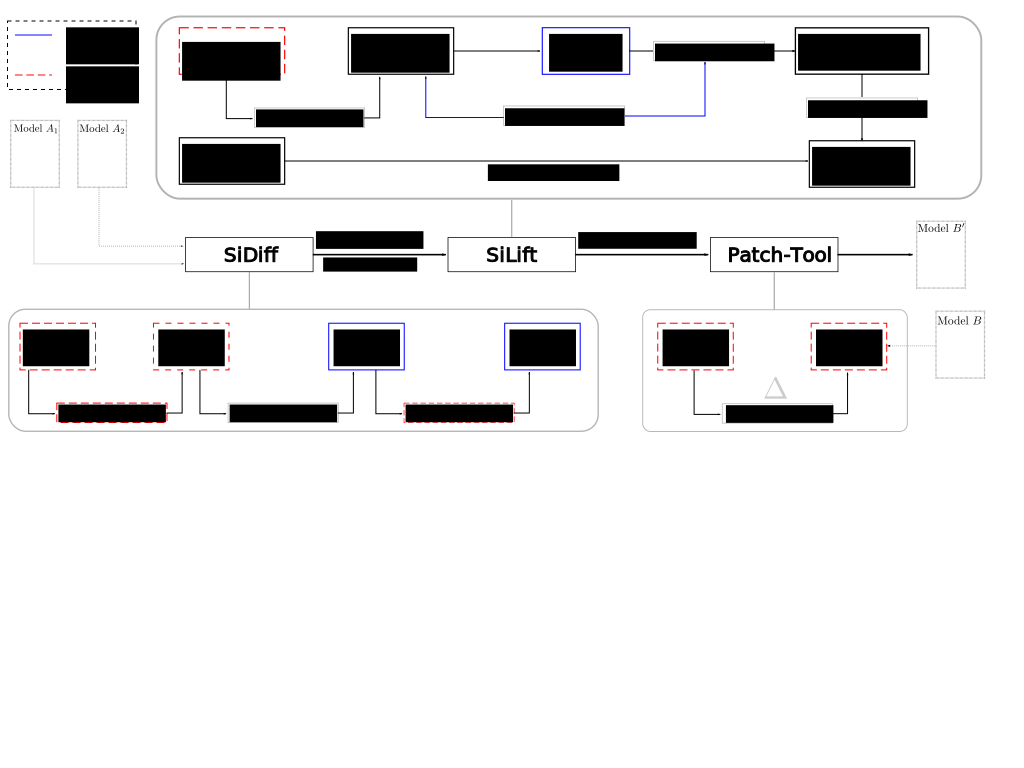
\includegraphics[scale=0.375]{integration_overview}\\
\end{center}
\end{frame}
\subsection{SiDiff}
\begin{frame}
\frametitle{Matching approaches}
To match \textbf{stereotyped} elements, there are two possible approaches:
\medskip
\begin{columns}[t]
 \column{0.5\textwidth} 
 \textbf{SiDiff Profile configuration}
\begin{itemize}
  \item[$+$] No new matching service has to be created
  \item[$-$] Profiled elements do not own much \glqq semantic\grqq\ meaning
  useful for similarity-based matching
  \item[$-$] Each UML Profile needs its own configuration
\end{itemize}
\column{0.5\textwidth}
 \textbf{Additional Matcher}
\begin{itemize}
 \item[$+$] No configuration necessary
 \item[$+$] All UML Profiles are generically supported
 \item[$+$] UML configuration is used for unprofiled elements
 \item[$-$] New matching service has to be created
\end{itemize}
\end{columns}
\end{frame}
\begin{frame}
\frametitle{Profiles matching example}
\begin{center}
Basic example for matching profiled elements: \\
\medskip
\includegraphics[scale=0.8]{profilematcher_example1}\\
\end{center}

\end{frame}
\begin{frame}
\frametitle{Profiles matching example}
\begin{center}
UUID-Matcher: Generic matching, no difference: \\
\medskip
\includegraphics[scale=0.8]{profilematcher_example2}\\
\end{center}

\end{frame}
\begin{frame}
\frametitle{Profiles matching example}
\begin{center}
Similarity-Matcher: Matching base elements: \\
\medskip
\includegraphics[scale=0.8]{profilematcher_example3}\\
\end{center}

\end{frame}
\begin{frame}
\frametitle{Profiles matching example}
\begin{center}
Similarity-Matcher: How to match profiled elements? \\
\medskip
\includegraphics[scale=0.8]{profilematcher_example4}\\
\end{center}

\end{frame}
\begin{frame}
\frametitle{ProfileMatcher approach}
\begin{center}
Profile-Matcher: Match according to base elements: \\
\medskip
\includegraphics[scale=0.8]{profilematcher_example5}\\
\end{center}
\end{frame}
\begin{frame}
\frametitle{ProfileMatcher}
\begin{center}
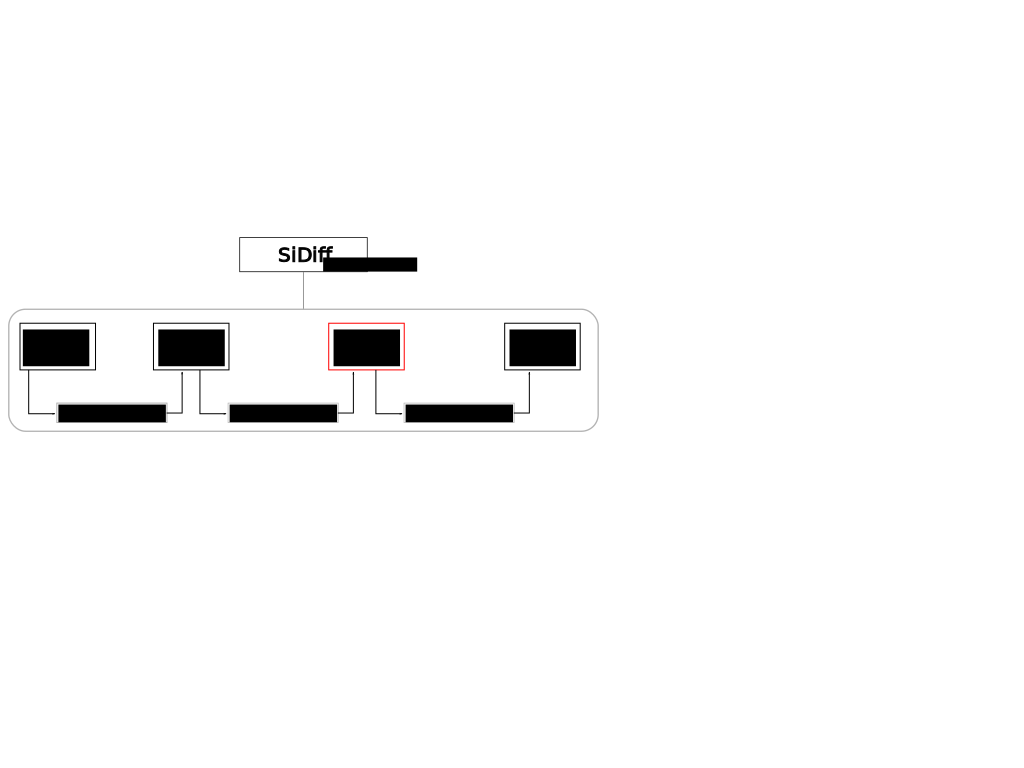
\includegraphics[scale=0.4]{profilematcher}\\
\end{center}
\begin{itemize}
  \item Implemented as a \textbf{SiDiff-Service}
  \item Can be \textbf{integrated} easily
  \item Used as \textbf{final} matching service for best results
  \item Makes use of \textbf{semantic} information of base elements of
  preceded matching services
  \item Depends on UML SiDiff \textbf{configuration}
\end{itemize}
\end{frame}
\begin{frame}
\frametitle{Wrong UUID example}
\begin{center}
\includegraphics[scale=0.32]{wrongUUIDs_examples_p3}\\
\end{center}

\end{frame}
\begin{frame}
\frametitle{UUID-Fixer}
\begin{center}
\includegraphics[scale=0.4]{uuidfixer}\\
\end{center}
\begin{itemize}
  \item Implemented as a \textbf{SiDiff-Service}
  \item Can be \textbf{integrated} easily
  \item Used as \textbf{final} SiDiff-service 
  \item SiDiff has only to be run once, UUID-Matcher is \textbf{sufficient}
  afterwards
  \item UUID-Fixing makes models \textbf{compatible} to other tools depending on
  right UUIDs
\end{itemize}
\end{frame}
\subsection{SiLift}
\begin{frame}
\frametitle{Edit Rule Profile integration approaches}
\begin{center}
\includegraphics[scale=0.6]{variants_overview}\\
\end{center}
\end{frame}
% \begin{block}{Approach 1: Generate rules directly}
% \begin{itemize}
%   \item[$+$] No additional tool needed, all done by \textbf{SERGe}
%   \item[$-$] Redundancy between UML rules and stereotyped rules
%   \item[$-$] Manual rules and corrections in UML rules are not carried over to
%   profiled rules
% \end{itemize}
% \end{block}
% \begin{block}{Approach 2: Combine base and stereotype rules}
% \begin{itemize}
%   \item[$+$] Manual rules and corrections in UML rules and stereotyped rules are
%   preserved
%   \item[$+$] Tool could be used in other areas (e.g. merging of atomic rules
%   into complex ones)
%    \item[$-$] Additional tool needed (for merging/combination)
%    \item[$-$] Time-consuming development approach
% \end{itemize}
% \end{block}
% \end{frame}
% \begin{frame}
% \frametitle{Edit Rule Profile integration approaches}
% \begin{block}{Approach 3: Transform base rules}
% \begin{itemize}
%   \item[$+$] Manual rules and corrections in UML rules are preserved
%   \item[$+$] Not as complex to develop as approach 2
%   \item[$+$] Academic bonus: Usage of Higher-Order-Transformations
%   \item[$-$] Additional tool needed (for transformating)
% \end{itemize}
% \end{block}
% \medskip
%  $\bm\triangleright$ ProfileApplicator implements approach \textbf{3}.
%\end{frame}

\begin{frame}
\frametitle{ProfileApplicator Overview}
\begin{center}
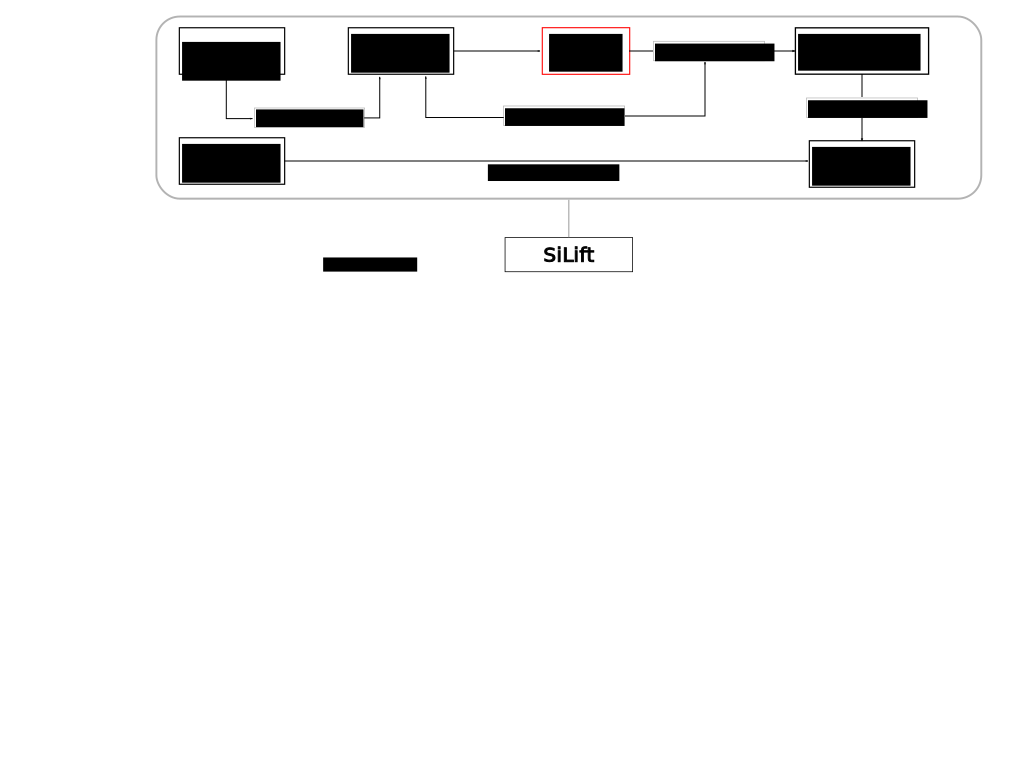
\includegraphics[scale=0.4]{profileapplicator}\\
\end{center}
\begin{itemize}
  \item Implemented as standalone \textbf{OSGi-Application}
  \item \textbf{Transforms} all files in given folder according to defined
  configuration via Higher-Order-Transformations
  \item \textbf{Minimal} configuration needed, more configuration options
  (Whitelist,\ldots) available
    \item Configuration and execution oriented after \textbf{SERGe} paradigms
\end{itemize}
\end{frame}
\begin{frame}
\frametitle{Higher-Order-Transformations}
\begin{itemize}
  \item Transforming Henshin Rules with Henshin Rules is called
  \textbf{Higher-Order-Transformation(HOT)}
  \item The ProfileApplicator is based on this feature of Henshin
  \item Henshin rules are defined as usual, but the elements to transform are
  elements of Henshin rules \textbf{itself}:
\end{itemize}
\begin{center}
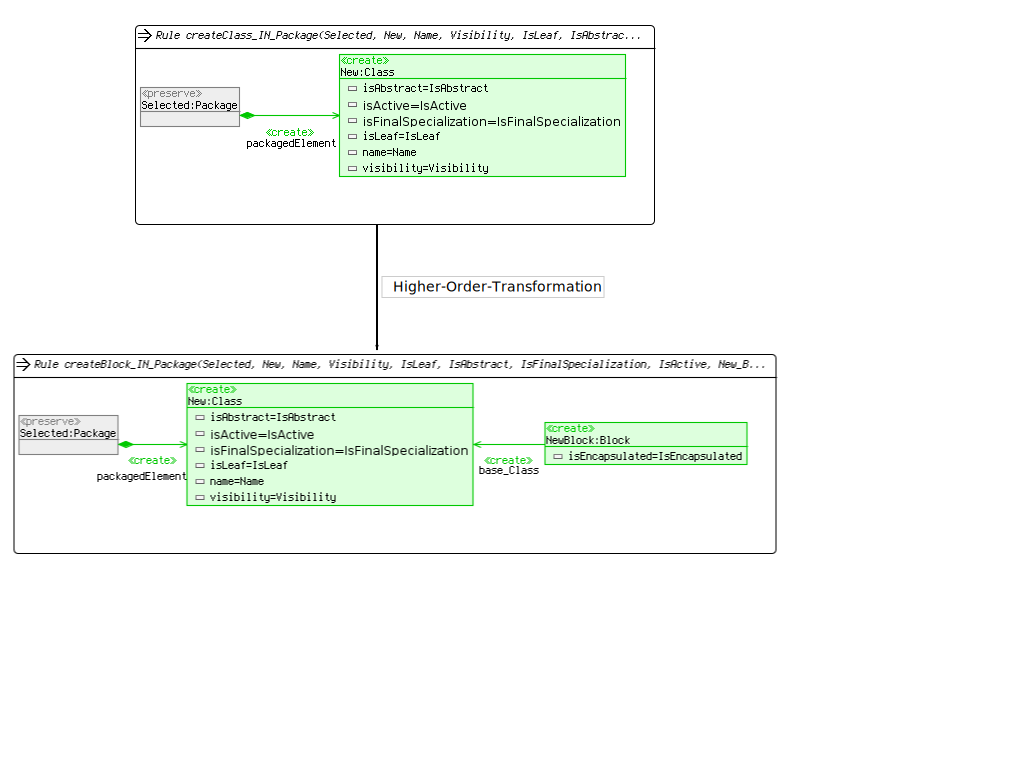
\includegraphics[scale=0.3]{hot_example}\\
\end{center}
\end{frame}
\begin{frame}
\frametitle{HOT for Create-Nodes}
\begin{center}
\includegraphics[scale=0.28]{CREATE_STEREOTYPE_IN_EDITRULE}\\
\end{center}
\end{frame}
\begin{frame}
\frametitle{HOT for Preserve-Nodes}
\begin{center}
\includegraphics[scale=0.3]{PRESERVE_STEREOTYPE_IN_EDITRULE}\\
\end{center}
\end{frame}
\begin{frame}
\frametitle{HOT for Delete-Nodes}
\begin{center}
\includegraphics[scale=0.35]{DELETE_STEREOTYPE_IN_EDITRULE}\\
\end{center}
\end{frame}
\begin{frame}
\frametitle{Complex edit rules}
\begin{center}
\includegraphics[scale=0.4]{complexeditrules}\\
\end{center}
\begin{itemize}
  \item For better lifting results the \textbf{domain} engineer can define
  complex edit rules:
  \begin{itemize}
    \item A complex edit rule \textbf{consists} of $2$ or more atomic edit rules
    \item Defines a \textbf{common} edit operation
    \item Are \textbf{optional} on the contrary to atomic edit rules
    \item Require very good \textbf{domain-specific} knowledge 
  \end{itemize}  
\end{itemize}
\end{frame}
\begin{frame}
\frametitle{Complex edit rule example}
\begin{center}
\includegraphics[scale=0.4]{CREATE_Block_Interacting_Via_FlowPorts}\\
\end{center}
\end{frame}
\subsection{Patching}
\begin{frame}
\frametitle{Patching integration}
\begin{center}
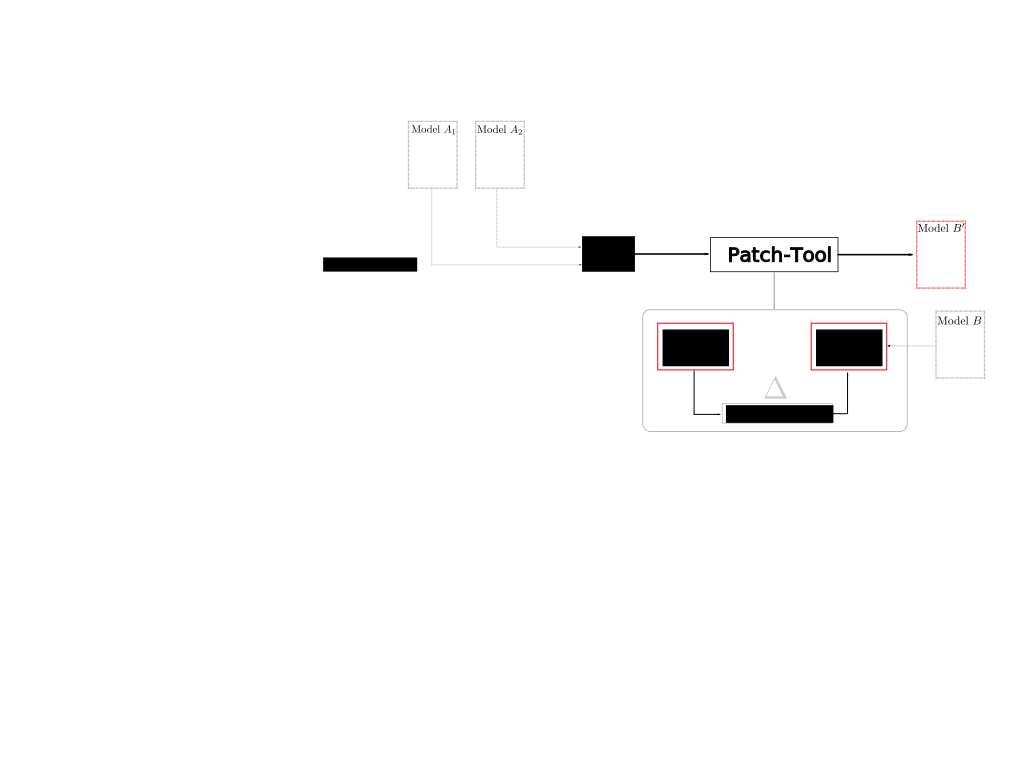
\includegraphics[scale=0.4]{patching}\\
\end{center}
\begin{itemize}
  \item For \textbf{creation} of patches all low-level changes must be (at
  least) lifted to atomic edit operations
  \item For \textbf{application} of patches all parameters of the patch must be
  set correctly
\end{itemize}
\end{frame}
\begin{frame}
\frametitle{Patching integration}
\begin{center}
\includegraphics[scale=0.4]{patching_correctness}\\
\end{center}
\begin{itemize}
  \item Model $B'$ needs to contain all \textbf{changes}
  between $A_1$ and $A_2$ for full \textbf{correctness}: \\
  \begin{center}
  If $B = A_1$ then $B' \overset{!}{=} A_2$ 
  \end{center}
\end{itemize}
\end{frame}
\section{Results}
\begin{frame}
\frametitle{General Results}
\begin{itemize}
  \item Between \textbf{all} revision changes can be:
  \begin{itemize}
    \item Matched
    \item Lifted
    \item Patched
  \end{itemize}
  \item \glqq Real World\grqq\ study is \textbf{considerably} larger and
  complexer than previous studies
  \item This leads to:
  \begin{itemize}
    \item Very \textbf{time consuming} calculations through all pipeline steps
    \item \textbf{Not} very accessible and easy to debug for edit rule engineer
    \item Good testing possibilities for \textbf{all} tools 
  \end{itemize}    
\end{itemize}
\end{frame}
\begin{frame}
\frametitle{Results for SysML case study}
\begin{center}
\includegraphics[scale=0.35]{revisionChanges_analysis}\\
\end{center}
\end{frame}
\begin{frame}
\frametitle{Results for SysML case study}
\begin{center}
{\small
\begin{tabular}{|c|c|c|c|c|}
\hline
Revision Change & Correspondences & Differences & Operations & Equal\\
\hline
00$\rightarrow$01 & 545 & 58 & 16  & {\color{green}Yes} \\
01$\rightarrow$02 & 545 & 203 & 86  & {\color{green}Yes} \\
02$\rightarrow$03 & 575 & 764 & 231  & {\color{green}Yes} \\
03$\rightarrow$04 & 774 & 9 & 9  & {\color{green}Yes} \\
04$\rightarrow$05 & 756 & 654 & 201  & {\color{green}Yes} \\
05$\rightarrow$07 & 904 & 165 & 102  & {\color{green}Yes} \\
07$\rightarrow$08 & 927 & 103 & 28  & {\color{green}Yes} \\
08$\rightarrow$09 & 943 & 298 & 94  & {\color{green}Yes} \\
09$\rightarrow$10 & 1008 & 367 & 111  & {\color{green}Yes} \\
10$\rightarrow$11 & 1099 & 83 & 28  & {\color{green}Yes} \\
11$\rightarrow$12 & 1107 & 436 & 143  & {\color{green}Yes} \\
12$\rightarrow$13 & 1216 & 95 & 40  & {\color{green}Yes} \\
\hline
\end{tabular}
}
\end{center}
\end{frame}

\section{Conclusion}
\begin{frame}
\frametitle{Summary}
UML Profiles integration into every pipeline step:
\begin{center}
\includegraphics[scale=0.375]{integration_overview_ready}\\
\end{center}
\end{frame}
\begin{frame}
\frametitle{Summary}
UML Profiles integration into every pipeline step:
\begin{center}
\includegraphics[scale=0.375]{integration_overview_ready_p1}\\
\end{center}

\end{frame}
\begin{frame}
\frametitle{Summary}
UML Profiles integration into every pipeline step:
\begin{center}
\includegraphics[scale=0.375]{integration_overview_ready_p2}\\
\end{center}
\end{frame}
\begin{frame}
\frametitle{Summary}
UML Profiles integration into every pipeline step:
\begin{center}
\includegraphics[scale=0.375]{integration_overview_ready_p3}\\
\end{center}

\end{frame}
\begin{frame}
\frametitle{Summary}
UML Profiles integration into every pipeline step:
\begin{center}
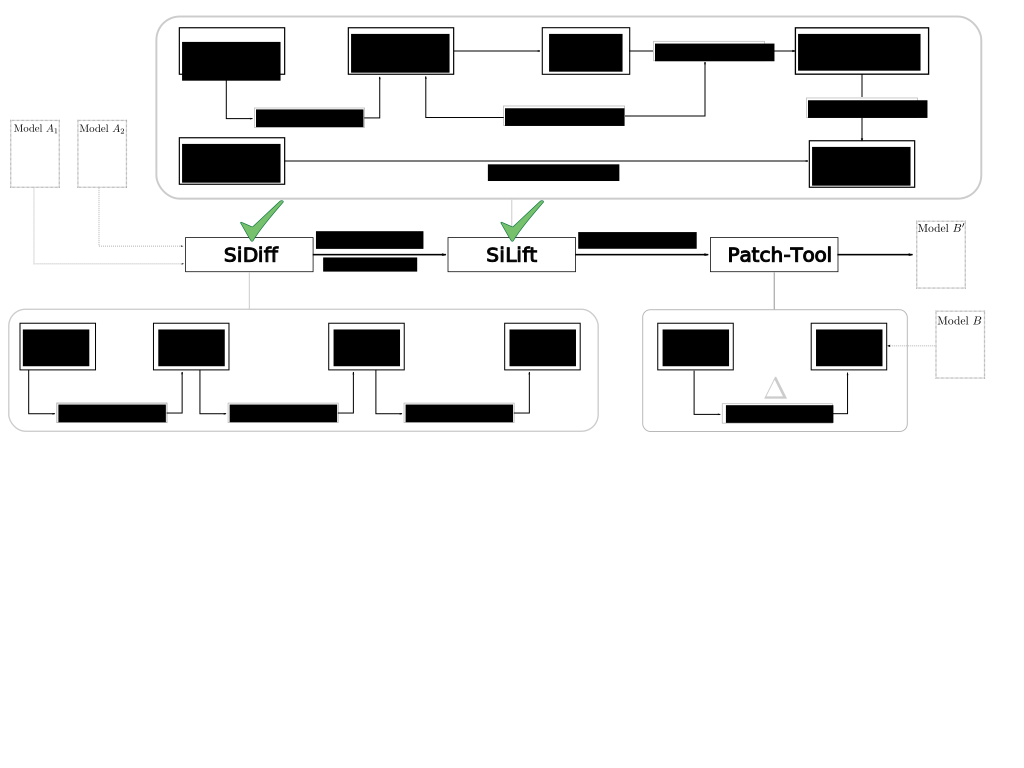
\includegraphics[scale=0.375]{integration_overview_ready_p4}\\
\end{center}
\end{frame}
\begin{frame}
\frametitle{Summary}
UML Profiles integration into every pipeline step:
\begin{center}
\includegraphics[scale=0.375]{integration_overview_ready_p5}\\
\end{center}

\end{frame}
\begin{frame}
\frametitle{Summary}
UML Profiles integration into every pipeline step:
\begin{center}
\includegraphics[scale=0.375]{integration_overview_ready_p6}\\
\end{center}
\end{frame}
\section{Future Work}
\begin{frame}
\frametitle{Outlook}
The following aspects could be considered in future work:
\begin{itemize}
  \item Extensive testing of implemented tools and services regarding other
  UML profiles like \textbf{MARTE}
  \item Construct more complex edit rules for better lifting results 
  \item Integrate approach \textbf{1} of profiling edit rules into
  \textbf{SERGe}
  \item Implement approach \textbf{2} of profiling edit rules as standalone tool
	with following features:
	\begin{itemize}
	  \item Combine base type edit rules with profiled ones
	  \item Combine \textbf{atomic} edit rules into \textbf{complex} edit rules
	  		without the need of manually creating the latter.
	 \end{itemize}
	\item Performance optimization for \textbf{large} and \textbf{real} models in
	all tools and pipeline steps
\end{itemize}
\end{frame}
\section{Literature}
\begin{frame}
\frametitle{Bibliography}
\bibliographystyle{alpha}
\bibliography{presentation}
\end{frame}
\end{document}